\documentclass[8pt,twocolumn]{article}
\usepackage{fullpage,amsmath,amsfonts,amssymb,color,tabularx}
\usepackage{enumerate,braket,cases,graphicx}
\usepackage{listings}
\usepackage{color}
\definecolor{mygreen}{rgb}{0,0.6,0}
\definecolor{mygray}{rgb}{0.5,0.5,0.5}
\definecolor{mymauve}{rgb}{0.58,0,0.82}
\lstset{
    basicstyle=\ttfamily\footnotesize,
    commentstyle=\color{mygreen},
    keywordstyle=\color{blue},
    language=Python,
    stringstyle=\color{mymauve}
}

\renewcommand{\vec}{\boldsymbol}
\newcommand{\mat}{\boldsymbol}
\newcommand{\tens}{\boldsymbol}

\newcommand{\I}{\mathrm{i}}
\newcommand{\e}{\mathrm{e}}
\newcommand{\D}{\mathrm{d}}

\usepackage{mathpazo}
\linespread{1.05}
\usepackage[T1]{fontenc}

\begin{document}
\twocolumn[
\begin{@twocolumnfalse}

\begin{center}
\textsc{AP3081D International Master Course on Computational Physics}\\
\textbf{Lattice Boltzmann\\
\today}\\
\end{center}
\begin{center}
Chiel Donkers, 1327704
\end{center}

\hrule
\begin{abstract}
The purpose of this paper is to report on the results obtained for a simple 1D flow in a tube using a Lattice Boltzmann code developed during the course. Where the density and the viscosity of the fluid is varied from $0.6 \le \rho \le 1.4$ and $0.033 \le \nu \le 0.133$. The simulations are coded in FORTRAN90.

The obtained results correspond to the known relationship $\Delta P / \left(\rho \nu \right)$.\\

\hrule
\end{abstract}

\end{@twocolumnfalse}]

\section*{Introduction}
The Lattice Boltzmann method is a special form of Compuational Fluid Dynamics (CFD). Instead of simulating large scale macroscopic properties, like most CFD codes, the Lattice Boltzmann method imposes a local equilibrium distribution at each point for every time step. 

Instead of placing particles on each gridpoint we only consider a distribution of densities in different directions. For every time step these densities are moved to their corresponding new gridpoints. Where any boundary conditions and external forces are imposed on the distribution. After which this distribution is relaxed to a new equilibrium distribution.

\section*{Code}
\begin{figure}[!b]
\centering
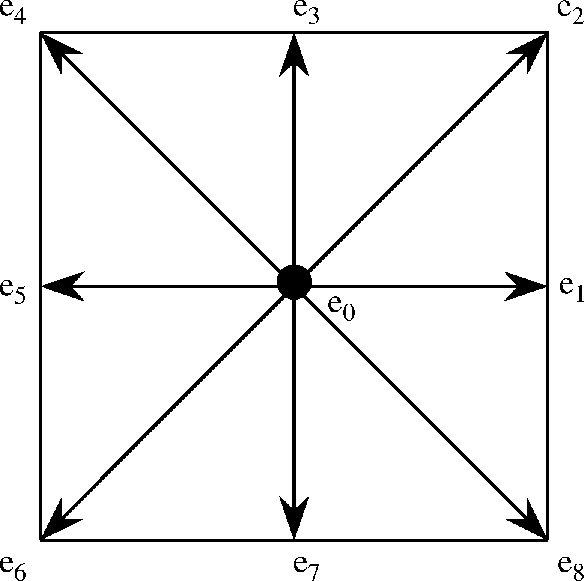
\includegraphics[width=0.8\linewidth]{images/d2q9.png}
\caption{The d2q9 grid used in the Lattice Boltzmann simulation with corresponding numbering.}
\label{fig:d2q9}
\end{figure}
The lattice used in the code is a d2q9 grid which can be viewed in Fiq.~\ref{fig:d2q9}. Here the numbers correspond to the possible particle velocities. For this grid the equilibrium distribution can be obtained using the formula,
\begin{equation}
n^{eq}_i = w_i \frac{\rho}{m} \left(1 + \frac{3}{c^2} e_{i\alpha}u_{\alpha} + \frac{9}{2c^4} e_{i\alpha}e_{i\beta}u_{\alpha}u_{\beta} - \frac{3}{2} \frac{u_{\alpha}u_{\alpha}}{c^2} \right)
\label{eq:neq}
\end{equation}
Here, $i$ labels the 9 possible directions with 0 the rest density, $\alpha$ and $\beta$ are Cartesian coordinates for $x$ and $y$. $w_i$ is a weighting factor for a specific direction given as,
\begin{equation}
w_i = 
  \begin{cases}
  4/9 & \text{for } i = 0 \\
  1/9 & \text{for } i = 1,3,5,7 \\
  1/36 & \text{for } i = 2,4,6,8
  \end{cases}
\label{eq:wi}
\end{equation}

To simulate a flow through a tube we need to implement the boundary conditions at the walls. The simplest way to define this is a 'stick' boundary condition which implies zero velocity at the walls. To obtain this a bounce back condition is used for any density that would otherwise leave the tube through one of the walls. This is implemented using a ghost cell that is placed outside the simulated area where any densities reaching this cell has it's velocity reversed. On average this results in a zero velocity between the ghost cell and the first cell of the simulated area.

For simulating the flow through the tube a small pressure gradient is applied from the left to the right. This is done by adding a small velocity along the direction of the gradient for every timestep.
In order to obtain the steady state solution in a short simulated tube periodic boundary conditions are applied to the left and right side.  

To obtain a smooth transition to the final steady state the newly obtained equilibrium density is averaged with the old equilibrium condition according to,
\begin{equation}
n^{new}_i = \left(1 - 1/\tau\right) n^{old}_i + n^{eq}_i/\tau
\label{eq:equil}
\end{equation}
\section*{Simulations and Results}
\begin{figure}[!b]
\centering
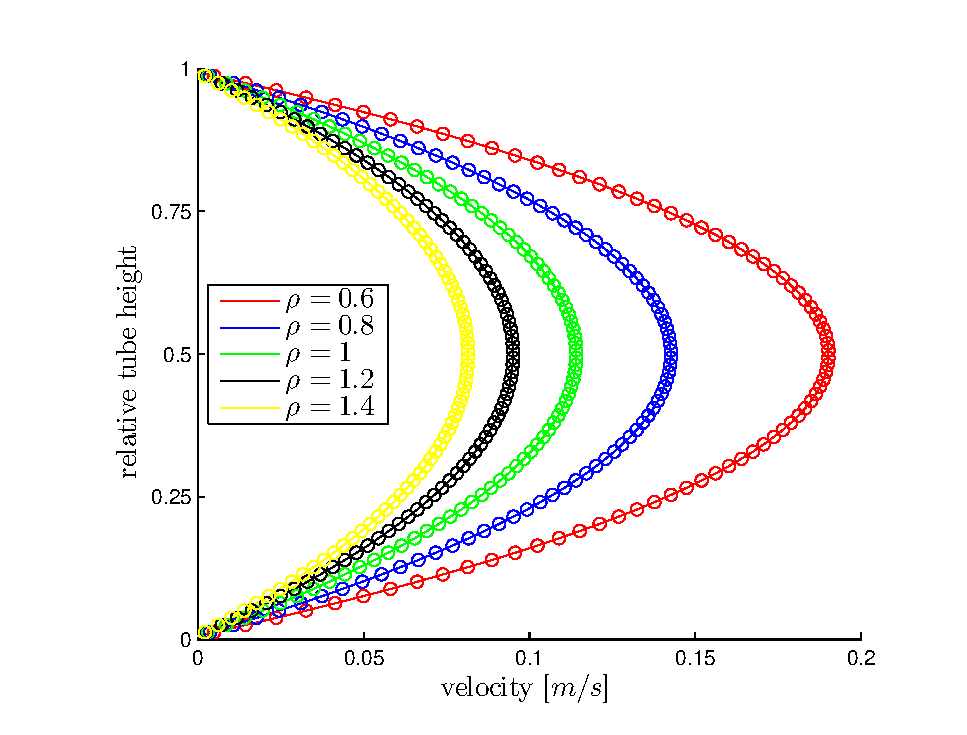
\includegraphics[width=\linewidth]{images/rho.eps}
\caption{Simulated results for various $\rho$, solid line represents second order polynomial fit of the simulated points represented as circles.}
\label{fig:rho}
\end{figure}
\begin{figure}[!b]
\centering
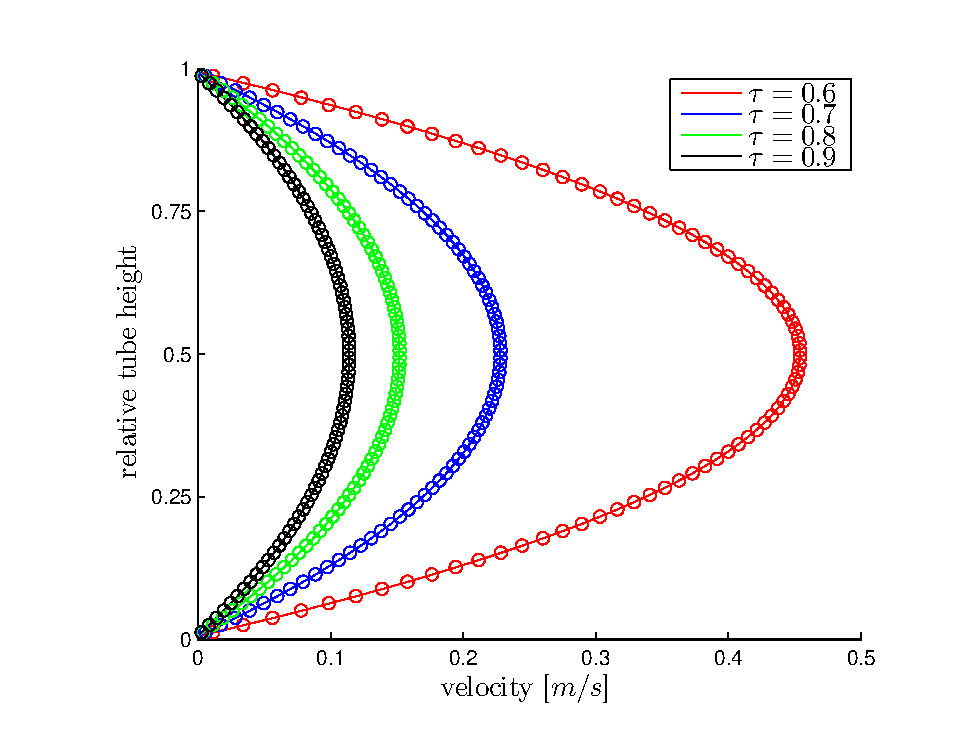
\includegraphics[width=\linewidth]{images/tau.eps}
\caption{Simulated results for various $\tau$, solid line represents second order polynomial fit of the simulated points represented as circles.}
\label{fig:tau}
\end{figure}

\begin{table}
\begin{center}
\setlength{\tabcolsep}{20pt}
\begin{tabular}{lcc}
 & fit & theory \\
\hline
$\rho = 0.6$ & 0.1249 & 0.1250 \\
$\rho = 0.8$ & 0.0937 & 0.0938 \\
$\rho = 1$   & 0.0749 & 0.0750 \\
$\rho = 1.2$ & 0.0624 & 0.0625 \\
$\rho = 1.4$ & 0.0535 & 0.0536 \\
\hline
$\tau = 0.6$ & 0.2975 & 0.3000 \\
$\tau = 0.7$ & 0.1496 & 0.1500 \\
$\tau = 0.8$ & 0.0998 & 0.1000 \\
$\tau = 0.9$ & 0.0749 & 0.0750
\end{tabular}
\end{center}
\label{tab:results}
\end{table}
\end{document}
